Pour améliorer nous allons construire des \textbf{fonctions} pour
\textbf{factoriser} les traitements et constituer une \textbf{chaîne
de traitement} fiable.

\textbf{Etape 1: lire}

Ce qui va changer ici c'est qu'on veut traiter plusieurs textes facilement.
Bien sûr on pourrait faire :

\begin{python} with open("13846-0.txt") as f:\#Discours de la Methode
chaine1 = f.read() with open("4300-0.txt") as f:\#Ulysses chaine2
= f.read() \end{python} La première chose que l'on remarque c'est
que sur Windows (le problème ne se pose pas avec Mac ou Linux) on
arrive à ouvrir le texte en anglais mais pas celui en français. C'est
un problème d'encodage des caractères (\texttt{charmap} error). L'encodage
c'est la manière dont on stocke les caractères en les changeant en
"0" et en "1". Pour faire simple, quand on a des caractères accentués
on a besoin d'un encodage (\textit{encoding}) adapté. Ici c'est "utf-8",
on va faire la modification suivante : \begin{python} with open("13846-0.txt",
encoding='utf-8') as f:\#Discours de la Methode chaine1 = f.read()

with open("4300-0.txt") as f:\#Ulysses chaine2 = f.read() \end{python}

On voit que l'on a répété deux fois le même code et aussi que si l'on
a des correctiosn à faire, il faudra le faire deux fois.

Si on a 100 textes à traiter il faut 300 lignes de code, pas très
pratique.Nous allons voir avec une fonction ça marche mieux. Pour
la fabriquer il faut décomposer notre problème, voir \textbf{ce qui
est constant} (factorisable, les opérations) et \textbf{ce qui est
variable} (non factorisable, paramètre ou sortie de la fonction).
On se rend vite compte que ce que l'on veut c'est à partir d'un chemin
de fichier (\textbf{input} ou entrant) avoir son contenu sous forme
de chaîne de caractères (\textbf{output} ou sortant). Ce qui nous
donne :

\begin{python} def lirefichier(chemin): with open(chemin, encoding
= 'utf-8') as f: chaine = f.read() return chaine

chaine1 = lirefichier("13846-0.txt")\#Discours de la Methode chaine2
= lirefichier("4300-0.txt")\#Ulysses

\end{python}

\textbf{Etape 2 : découper}

Toujours réfléchir en terme d'entrant/sortant : Quel est l'entrant
et le sortant qu'il faut ajouter dans le squelette ci-contre à la
place des XXX, YYY et ZZZ?

\begin{python} def decouperenmots(XXX): \#on decoupe listemots =
YYY return ZZZ

\end{python}

(à vous de réfléchir, réponse page suivante) \newpage{}

\begin{python} def decouperenmots(chaine): \#on decoupe listemots
= chaine.split() return listemots

listemots1 = decouperenmots(chaine1) listemots2 = decouperenmots(chaine2)
\end{python}

\textbf{Etape 3 : compter}

En entrée : la liste de mots

En sortie : les effectifs

NB: vous pouvez mettre des \textit{print} quand vous testez pour bien
voir ce qu'il se passe.

\begin{python}

def geteffectifs(listemots): diclongueurs = {} for mot in listemots:
longueur = len(mot)\#la longueur du mot if longueur not in diclongueurs:
\#on a jamais vu cette longueur de mot diclongueurs{[}longueur{]}=1
\# else: \#on a vu cette longueur de mot diclongueurs{[}longueur{]}+=1
return diclongueurs

\end{python}

Et cette fonction on va l'utiliser directement dans l'étape 5

\textbf{Etape 4 : observer (obsolète)}

C'était une étape de vérification devenue inutile puisqu'on n'a pas
changé les opérations effectuées.

\textbf{Etape 5 : représenter}

Ici on va pouvoir afficher les deux courbes sur la même figure et
cerise sur le gâteau on va la sauvegarder.

\begin{python} import matplotlib.pyplot as pyplot \#import avec alias

for liste in {[}listemots1, listemots2{]}: \#on a une liste de liste
pour factoriser diclongueurs = geteffectifs(liste) listeeffectifs
= {[}{]} for toto in range(30): if toto in diclongueurs:\#on a donc
vu des mots de cette longueur listeeffectifs.append(diclongueurs{[}toto{]})
else:\#on en n'a pas vu de cette longueur, on ajoute donc un 0 listeeffectifs.append(0)
pyplot.plot(listeeffectifs)\#on "dessine" mais dans la boucle

pyplot.show()\#"on affiche" mais hors de la boucle (pour avoir tout)

\end{python}

\begin{figure}
\centering{}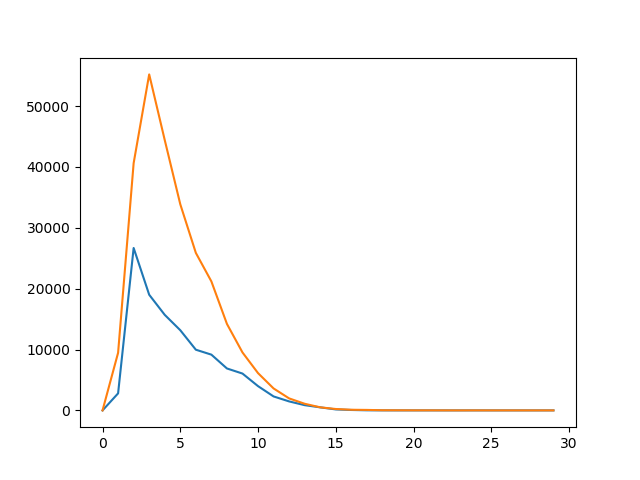
\includegraphics[width=0.5\textwidth]{images/TD1_effectifs_total.png}
\caption{"Discours de la Méthode" et "Ulysses" : nombre de mots par longueur
(en abscisse), en ordonnée l'effectif}
\end{figure}

On se rend compte que la figure est difficile à interpréter, en effet
on travaille en valeur absolue alors que les textes sont de taille
différente. On va donc utiliser la taille de chaque texte en mots
(avec la fonction \texttt{len}) pour avoir cette fois une figure avec
la proportion de mots de chaque longueur :

\newpage{}

\begin{python} \#On remplace la ligne : listeeffectifs.append(diclongueurs{[}toto{]})
\#Par: listeeffectifs.append(diclongueurs{[}toto{]}/len(liste)) \end{python}

\begin{figure}
\centering{}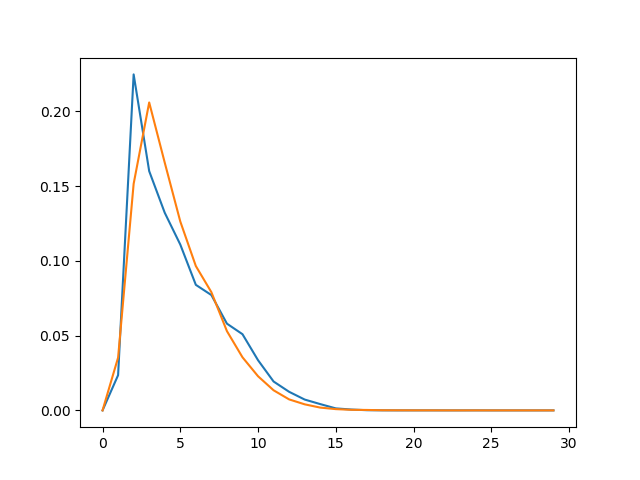
\includegraphics[width=0.5\textwidth]{images/TD1_frequences_total.png}
\caption{"Discours de la Méthode" et "Ulysses" : nombre de mots par longueur
(en abscisse), en ordonnée la fréquence}
\end{figure}

Voir page suivante pour un bilan

\newpage\textbf{Après une dernière étape de factorisation voici où
nous en sommes :}

\begin{python} def lirefichier(chemin): with open(chemin, encoding
= "utf-8") as f: chaine = f.read() return chaine

def decouperenmots(chaine): listemots = chaine.split() return listemots

def geteffectifs(listemots): diclongueurs = {} for mot in listemots:
longueur = len(mot) if longueur not in diclongueurs: diclongueurs{[}longueur{]}=1
else: diclongueurs{[}longueur{]}+=1 return diclongueurs

def vecteurlongueurs(diclongueurs, listemots): listeeffectifs = {[}{]}
for toto in range(30): if toto in diclongueurs: listeeffectifs.append(diclongueurs{[}toto{]}/len(listemots))
else: listeeffectifs.append(0) return listeeffectifs

import matplotlib.pyplot as pyplot

for chemin in {[}"13846-0.txt", "4300-0.txt"{]}: chaine = lirefichier(chemin)
listemots = decouperenmots(chaine) diclongueurs = geteffectifs(listemots)
listeeffectifs = vecteurlongueurs(diclongueurs, listemots) pyplot.plot(listeeffectifs)

pyplot.savefig("frequences.png")\#le bonus: on sauvegarde pyplot.show()

\end{python}

C'est pas mal, au prochain TD on améliorera le rendu de la figure
(légende, échelle) et on travaillera sur plus de langues. 
